\section{Eficiência}
\label{sec:eficiencia}

\subsection{Análise do custo}
\label{sec:custo}

Seja $N$ o lado do tabuleiro. Há $V = N^2$ casas, e cada casa tem no máximo 8 pulos, então o
grafo tem $E \le 8N^2$ arestas.

\textbf{Tempo.} O trabalho do Algoritmo~\ref{alg:bfs} é contado por partes:

\begin{itemize}
  \item A inicialização de $dist$ (linha~\ref{lin:init}) percorre todas as casas:
    $\Theta(N^2)$.
  \item Cada casa entra na fila no máximo uma vez, porque só entra se $dist$ ainda vale $-1$
    (linha~\ref{lin:novo}) e é marcada na hora (linha~\ref{lin:marca}). Logo, o laço da
    linha~\ref{lin:while} roda no máximo $N^2$ vezes.
  \item A cada volta, o laço da linha~\ref{lin:for} executa exatamente 8 vezes (o
    Algoritmo~\ref{alg:pulos} sempre devolve 8 pares), e cada execução faz um número constante
    de operações: duas somas, dois módulos, uma consulta e uma atualização em $dist$ e uma
    inserção na fila, todas em tempo constante.
\end{itemize}

Somando, o laço principal faz no máximo $N^2 \times 8 \times c$ operações, para uma constante
$c$, ou seja, $O(N^2)$. Em termos de vértices e arestas, é o custo $\Theta(V + E)$ conhecido da
BFS~\cite{cormen}. Como a inicialização já custa $N^2$ em qualquer tabuleiro, o tempo do
algoritmo é $\Theta(N^2)$ sempre. O que muda de um tabuleiro para outro é a constante: quando S
é encontrada cedo, a busca visita só parte das casas.

\textbf{Espaço.} A matriz $dist$ ocupa $N^2$ inteiros, a fila guarda no máximo $N^2$ casas
(cada uma entra uma vez) e o próprio tabuleiro ocupa $N^2$ caracteres. O espaço é, portanto,
$\Theta(N^2)$.

Não dá para melhorar a \emph{ordem de grandeza}: só para localizar S no tabuleiro, qualquer
algoritmo precisa, no pior caso, olhar as $N^2$ casas. A BFS é, então, assintoticamente ótima
para este problema, e os ganhos que restam são de constante (Seção~\ref{sec:conclusao}).

\subsection{Conferência com as medições}
\label{sec:medicoes}

Se o custo é proporcional a $N^2$, dobrar $N$ deve multiplicar o tempo por 4. Para conferir,
mede-se o pior caso: uma busca que não para em S e visita todas as casas alcançáveis. Isso
isola o efeito do tamanho do tabuleiro, sem depender de onde S está.

As medições foram feitas em um Apple M2 com 16~GB de memória, macOS 26.7 e Java 24.0.1, sem contar a
leitura do arquivo. Cada tempo é o melhor de 15 execuções na mesma JVM, o que descarta o custo de
compilação das primeiras execuções e a interferência da coleta de lixo. Também se fixou o
tamanho da memória da JVM (\texttt{-Xms2g -Xmx2g}): com tamanho automático, o tempo absoluto
variou em até 1,8 vez de uma execução para outra, mas as razões entre tamanhos, que são o que
se usa aqui, não mudaram.

\begin{table}[ht]
  \centering
  \caption{Exploração completa, sem parar em S. As duas últimas colunas comparam cada tamanho
  com o anterior: se o custo é proporcional a $N^2$, elas devem ser parecidas.}
  \label{tab:crescimento}
  \small
  \begin{tabular}{|c|r|r|c|c|c|}
    \hline
    \textbf{$N$} & \textbf{Casas alcançadas} & \textbf{Tempo (ms)} & \textbf{ns por casa}
      & \textbf{Tempo / anterior} & \textbf{$N^2$ / anterior}\\
    \hline
    40 & 1.600 & 0,14 & 88 & - & -\\
    \hline
    80 & 6.398 & 0,62 & 96 & 4,4 & 4,0\\
    \hline
    100 & 9.999 & 0,97 & 97 & 1,6 & 1,6\\
    \hline
    150 & 22.494 & 2,23 & 99 & 2,3 & 2,3\\
    \hline
    200 & 39.992 & 4,02 & 101 & 1,8 & 1,8\\
    \hline
    400 & 159.950 & 16,41 & 103 & 4,1 & 4,0\\
    \hline
    800 & 639.857 & 67,35 & 105 & 4,1 & 4,0\\
    \hline
    1500 & 2.249.516 & 241,98 & 108 & 3,6 & 3,5\\
    \hline
  \end{tabular}
\end{table}

A Tabela~\ref{tab:crescimento} confirma a previsão: a razão entre os tempos acompanha a razão
entre os valores de $N^2$ em todos os tamanhos. O tempo por casa visitada, que deveria ser
constante, sobe pouco, de 88 para 108 ns (23\%), enquanto o número de casas cresce 1400 vezes.
Uma hipótese para essa pequena alta é o uso de memória: o maior tabuleiro ocupa dezenas de
megabytes, que não cabem nos caches do processador; isso não foi medido. Para $N \le 100$ os
tempos ficam abaixo de 1~ms, perto do limite do que o cronômetro e a JVM medem com precisão, e
as razões desses tamanhos devem ser lidas com cuidado.

\begin{figure}[ht]
  \centering
  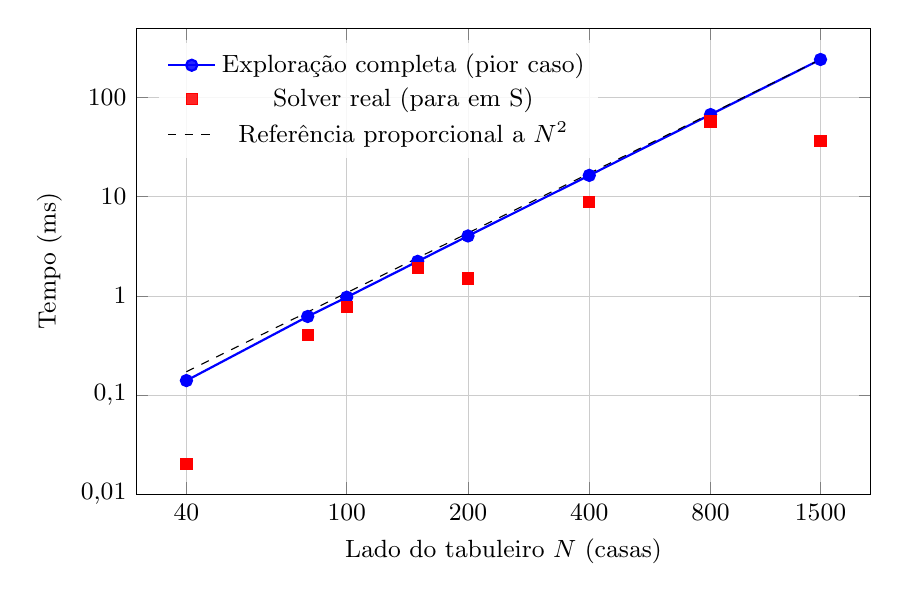
\begin{tikzpicture}
    \begin{loglogaxis}[
        width=0.9\linewidth, height=7.5cm,
        xlabel={Lado do tabuleiro $N$ (casas)},
        ylabel={Tempo (ms)},
        xmin=30, xmax=2000, ymin=0.01, ymax=500,
        xtick={40,100,200,400,800,1500}, xticklabels={40,100,200,400,800,1500},
        ytick={0.01,0.1,1,10,100}, yticklabels={0{,}01,0{,}1,1,10,100},
        xminorticks=false, yminorticks=false,
        grid=major, grid style={line width=0.2pt,draw=gray!40},
        tick label style={font=\small}, label style={font=\small},
        legend pos=north west,
        legend style={font=\small,draw=none,fill=white,fill opacity=0.85,text opacity=1},
      ]
      \addplot[mark=*,thick,blue] coordinates {
        (40,0.14) (80,0.62) (100,0.97) (150,2.23) (200,4.02) (400,16.41) (800,67.35) (1500,241.98)
      };
      \addlegendentry{Exploração completa (pior caso)}
      \addplot[only marks,mark=square*,red] coordinates {
        (40,0.02) (80,0.40) (100,0.78) (150,1.92) (200,1.50) (400,8.79) (800,57.24) (1500,36.30)
      };
      \addlegendentry{Solver real (para em S)}
      \addplot[dashed,black,domain=40:1500,samples=2] {241.98*(x/1500)^2};
      \addlegendentry{Referência proporcional a $N^2$}
    \end{loglogaxis}
  \end{tikzpicture}
  \caption{Tempo de execução por tamanho do tabuleiro, em escala logarítmica nos dois eixos. A
  exploração completa acompanha a reta tracejada, proporcional a $N^2$, que passa pelo ponto
  $N = 1500$. Os pontos vermelhos são os casos reais, em que a busca para ao chegar a S.}
  \label{fig:crescimento}
\end{figure}

\subsection{Por que os casos reais não crescem de forma regular}
\label{sec:casos-reais}

Nos casos reais o algoritmo para ao retirar S da fila, e o trabalho depende de onde S está em
relação a C. A Tabela~\ref{tab:resultados} mostra que a busca retira da fila desde 16,7\% das
casas (caso 1500) até 93,3\% (caso 800). Por isso o caso 1500, que tem 3,5 vezes mais casas
que o caso 800, é resolvido mais rápido (36,30~ms contra 57,24~ms): a BFS chega a S depois de
visitar uma parte pequena do tabuleiro, e o resto nem chega a ser explorado. É por isso que os
pontos vermelhos da Figura~\ref{fig:crescimento} ficam abaixo da curva do pior caso e não
seguem uma reta.
